
\section{Artstyle}\label{sec:artstyle}

\renewcommand{\kapitelautor}{Autor: Philip Jankovic}
%TODO quellen, verweis, bilder und rechtschreibung

\FF in game visuals sind handgezeichnet und oft statisch. Beim Zeichnen wurde zuerst eine "Reference" gesucht.


\subsection{References}\label{subsec:references}
References beim Zeichnen sind Bilder oder andere Artworks an denen sich orientiert wird. Vorallem am Anfang ist das
Arbeiten mit References fast ein Muss, da das einfache Vorstellen der Zeichnung im Kopf und das anschließende Zeichnen davon höchst anspruchsvoll ist.
Die Perspektive, Kleidung und Körperposen können von der Reference inspieriert werden.
Jedoch wird versucht die Reference nicht 100\% abzuzeichnen, sondern auch den eigenen Stil hinzufügen. \zit{referance}


Für \FF wurden References von "Pinterest", jedoch auch Inspirationen aus diversen Filmen und anderen Medien gesucht. \zit{pinterest}


Ein Beispiel für die Nutzung verschiedenster References ist der Manga \quoted{JOJO's Bizzzar Adventure} von Hirohiko Araki\zit{jojo},
welcher auch eine Inspiration für einige Teile von \FF ist. Nicht nur im Bezug auf die Zeichnungen, sondern auch auf die von dem Autor benützen Krativfindungsmethoden.
Mehr dazu kann in dem Kapitel \ref{methoden} gelesen werden.
Araki verwendet eine große Auswahl als References für seine Zeichnungen, vorallem aus der Welt
der Fashion, was auch in seinem Artstyle zu sehen ist.


\FF bezieht euch ein paar References von "JOJO's Bizzzar Adventure", jedoch ist die Auswahl der benützen References groß und abweichslungsreich.
Auch eigene selbst aufgenomme Reference-Bilder wurden verwenedet für \zB den Main-Charackter des Spieles.





Bei dem Nutzen einer Reference muss jedoch darauf geachtet werden, das Bild nicht nur abzuzeichnen. Je nach Zeichenstil
oder wie stilisiert ein Zeichenstil ist, besteht eine Gefahr, ein Bild nur abzuzeichnen, anstatt es als Reference zu verwenden.
Das Bewahrens eines eigenen Zeichenstiles ist dabei besonders wichtig.


\subsection{Artsytle von \FF}\label{subsec:artsytle}

Der Artstyle von \FF ist im Comic-stil gehalten, mit groben, Bleistift Outlines und Coloring auf der Ebene darunter.
Coloring wird mit einem Farbpinsel auf 100\% Fluss gemacht, damit die Kanten schön hart sind und es sich besser von dem Hintergrund abheben.
Auch wenn die Zeichnungen selber nicht realistisch gezeichnet sind, halten sie sich an realistische Posen und Propertionen, sind also nicht wirklich stilisiert.
Das Spiel nimmt sich dadurch nicht zu ernst, passt aber gut zu dem rauen Wild-West Setting und schlägt für den Betrachter trotz all dieser komischen Bullets
einen Anker in der Realität.

\begin{figure}[H]
    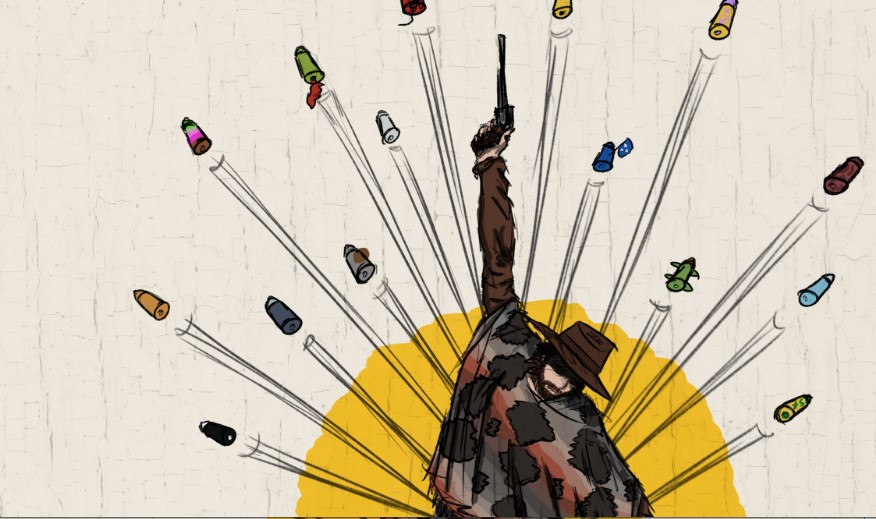
\includegraphics[width=50\%]{artstylepic.jpg}
    \caption{Beispiel: Artstyle von \FF}
\end{figure}


Um den Zeichnungen mehr Tiefe zu geben wird über der Color-Ebene eine Muliplate-Ebene auf 50\% Oppacity verwendet um Schatten
darzustellen. Geshaded wird mit dem selben Pinsel mit welchem Gecolored wird. Das Shading bleibt bei diesem einen grauen ton,
härtere shadows werden durch "Crosshatching" mit dem Outline-Bleistift gemacht.\zit{crosshatching}

\begin{figure}[H]
    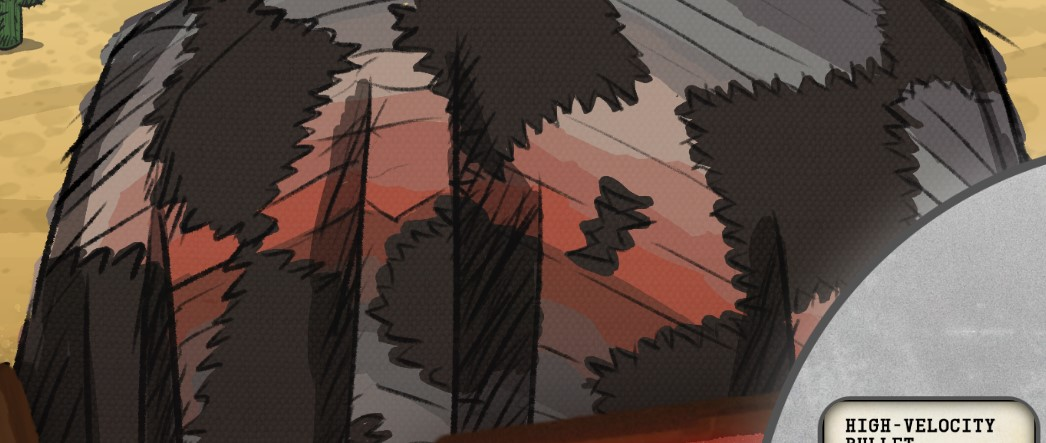
\includegraphics[width=50\%]{crossha.jpg}
    \caption{Beispiel: Crosshatching in \FF}
\end{figure}

%
% evolution der artstyles


%artstyle
%

% resets author
\renewcommand{\kapitelautor}{}
